%%%%%%%%%%%%%%%%%%%%%%%%%%%%%%%%%%%%%%%%%%%%%%%%%%%%%%%%%%%%%%%%%%%%%%
% LaTeX Template: Beamer arrows
%
% Source: http://www.texample.net/
% Feel free to distribute this template, but please keep the
% referal to TeXample.net.
% Date: Nov 2006
% 
%%%%%%%%%%%%%%%%%%%%%%%%%%%%%%%%%%%%%%%%%%%%%%%%%%%%%%%%%%%%%%%%%%%%%%
% How to use writeLaTeX: 
%
% You edit the source code here on the left, and the preview on the
% right shows you the result within a few seconds.
%
% Bookmark this page and share the URL with your co-authors. They can
% edit at the same time!
%
% You can upload figures, bibliographies, custom classes and
% styles using the files menu.
%
% If you're new to LaTeX, the wikibook is a great place to start:
% http://en.wikibooks.org/wiki/LaTeX
%
%%%%%%%%%%%%%%%%%%%%%%%%%%%%%%%%%%%%%%%%%%%%%%%%%%%%%%%%%%%%%%%%%%%%%%

\documentclass{beamer} %
\usetheme{CambridgeUS}
\usepackage[latin1]{inputenc}
\usefonttheme{professionalfonts}
\usepackage{times}
\usepackage{tikz}
\usepackage{amsmath}
\usepackage{verbatim}
\usetikzlibrary{arrows,shapes}



\author{Paul lindt \& Ali Saleh}
\title{Collaborative Video streaming for Mobile Devices}

\begin{document}

\begin{comment}
:Title: Beamer arrows
:Tags: Remember picture, Beamer, Physics & chemistry, Overlays
:Use page: 3

With PGF/TikZ version 1.09 and later, it is possible to draw paths between nodes across
different pictures. This is a useful feature for presentations with the
Beamer package. In this example I've combined the new PGF/TikZ's overlay feature
with Beamer overlays. Download the PDF version to see the result.

**Note.** This only works with PDFTeX, and you have to run PDFTeX twice.

| Author: Kjell Magne Fauske

\end{comment}

\frame {
\titlepage
}
% For every picture that defines or uses external nodes, you'll have to
% apply the 'remember picture' style. To avoid some typing, we'll apply
% the style to all pictures.
\tikzstyle{every picture}+=[remember picture]

% By default all math in TikZ nodes are set in inline mode. Change this to
% displaystyle so that we don't get small fractions.
\everymath{\displaystyle}
\section[Outline]{}
\frame{\tableofcontents}
\section{Introduction}
\subsection{Motivation/Problem}
\begin{frame}
\frametitle{Motivation/Problem}
\begin{itemize}
\item Growing demand for mobile Video Streaming
	\begin{itemize}
    	\item Mobile video more than 50\% of data traffic % cisco visual network index        
        \item Increasing device capabilities leading to higher data rates \\ (e.g. 4k displays)    
    \end{itemize}    
        \item A user can not use the entire bandwidth of the cell 		even if he is alone [1]
    \item Signal coverage fluctuation [2]
    \begin{itemize}
    	\item Changing distance to base station        
        \item External interference
        \item Multi-path propagation %cite wolfinger slides here
    \end{itemize}        
\end{itemize}


\end{frame}
\subsection{Overview of Solution}
\begin{frame}
\frametitle{What is ColStream}
\begin{itemize}
\item {\bf Col}laborative {\bf Stream}ing
\item Working prototype
\item Authors: Mingyang Zhong, Peizhao Hu, Jadwiga Indulska, Mohar J Kumar
\item Still in development
\item Focus on mobile scenario
\end{itemize}
\end{frame}

\section{Working Structure}
\begin{frame}
\frametitle{Technical Detail}
\begin{figure}[hbtp]
\centering
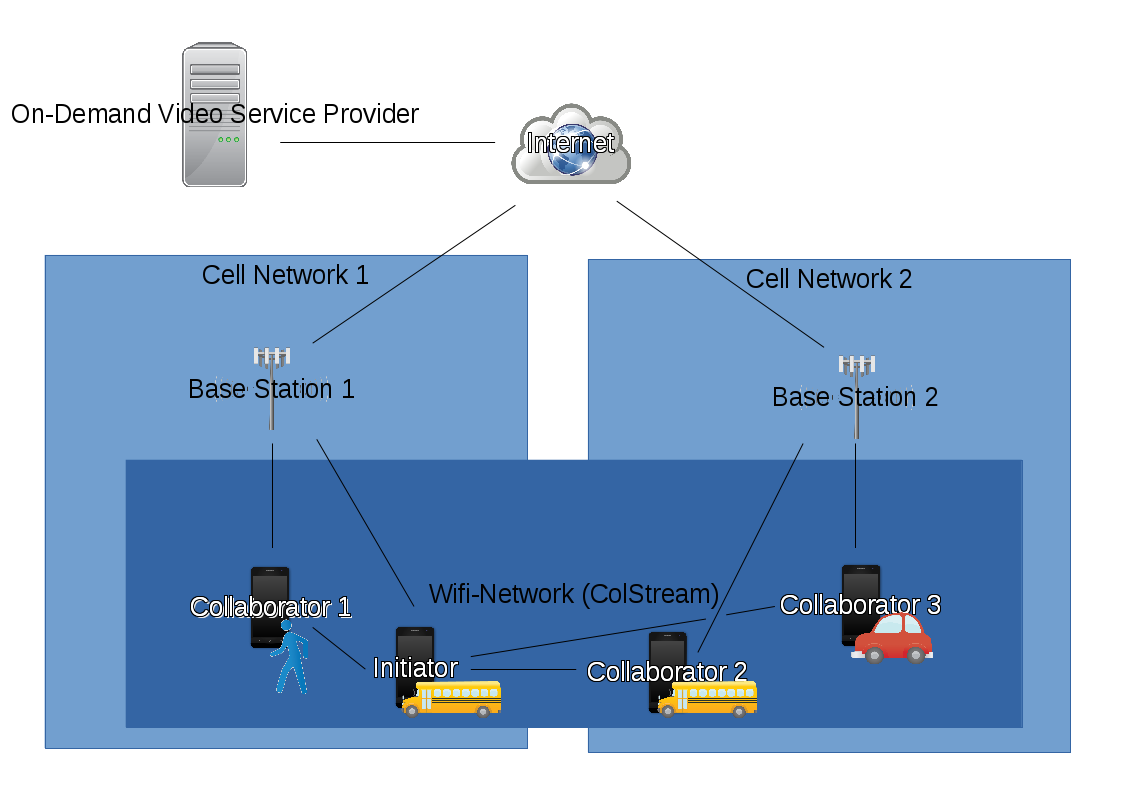
\includegraphics[scale=.35]{figures/Overview.png}
%\caption{Overview of the idea of ColStream}
\end{figure}


\end{frame}
\subsection{Collaborative Download}
\begin{frame}
\frametitle{Collaborative Download}
%Workflow for the structure of collaboration
\begin{figure}[hbtp]
\centering
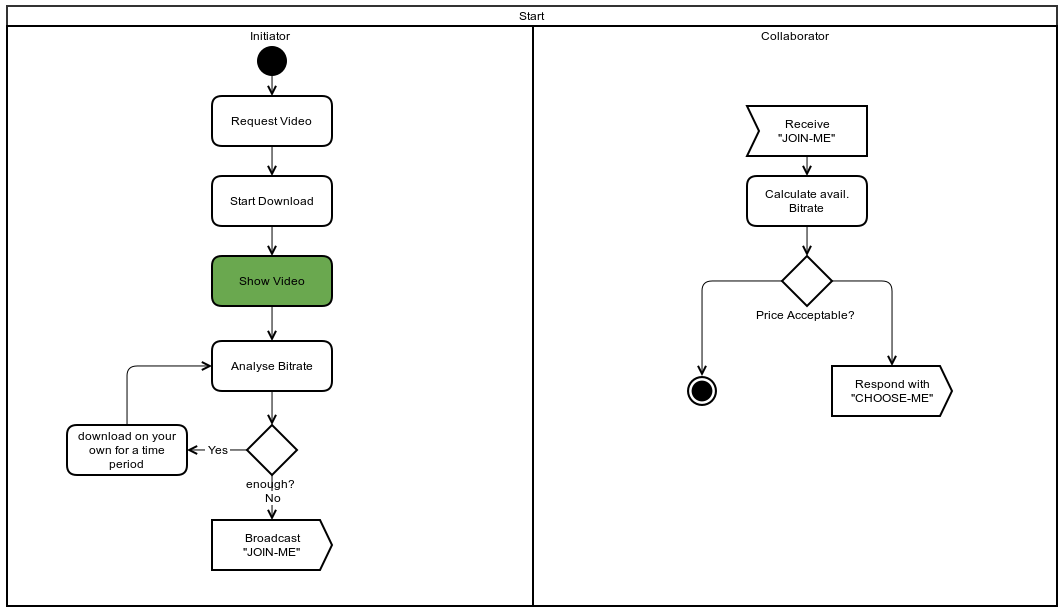
\includegraphics[scale=.4]{figures/Workflow_1.png}
\end{figure}
\end{frame}

\begin{frame}
\frametitle{Collaborative Download Cont.}
%Workflow for the structure of collaboration
\begin{figure}[hbtp]
\centering
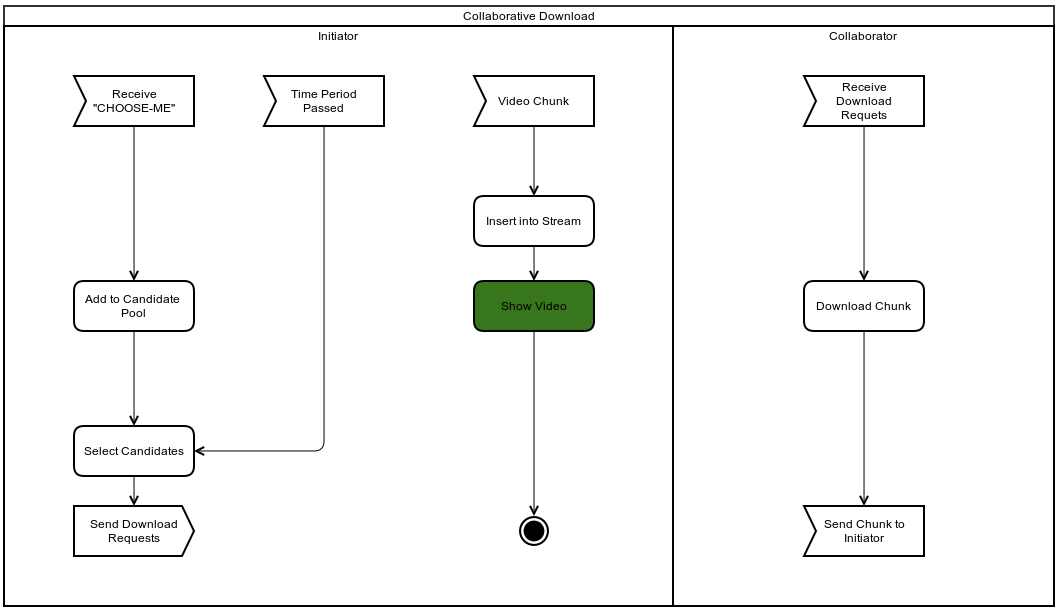
\includegraphics[scale=.4]{figures/Workflow_2.png}
\end{figure}
\end{frame}

\begin{frame}
\frametitle{Group Formation}
\begin{itemize}
\item Streaming begin initially
\item Background service check for bandwidth
\item \textit{JOIN-ME} message sent to nearby devices
\begin{itemize}
\item with contact information, purchase price, \& public key
\end{itemize}
\item Interested devices reply with \textit{CHOOSE-ME} message
\begin{itemize}
\item With estimated throughput of the connection and the selling price.
\end{itemize}
\item Collaborators pool is formed.
\end{itemize}
\end{frame}

\subsection{Working Algorithm}
\begin{frame}
\frametitle{Collaborators Selection}
Bandwidth estimation
\begin{itemize}
\item Collaborator periodically measured signal and achieved throughput
\item Those results are smoothed to avoid fluctuation 
\begin{itemize}
\item $signal=\alpha * signal_{new}+(1-\alpha)* signal_{old}$
\item $tp=\alpha * tp_{new}+(1-\alpha)* tp_{old}$
\end{itemize}
\item Those measures are used to asses the signal history of a collaborator.
\end{itemize}
\end{frame}

\begin{frame}
\frametitle{Collaborators Selection Cont.}
%pricing scheme
\begin{itemize}
\item User Specify it's own price per data unit
\item Price takes into account data usage and battery usage
\item The paper doesn't specify what is the price or how it get paid
\end{itemize}
\textbf{Choosing collaborator:}
\begin{itemize}
\item Multi-objective optimization problem is formulated
\end{itemize}
\end{frame}

\begin{frame}
\frametitle{Dynamic Work Distribution}
\begin{itemize}
\item Each collaborator assigned a chunk of the video to download
\item Chunk size is not fixed , it depends on the estimated throughput
\begin{itemize}
%{\frac{{MAX_CHUNK_SIZE * tp_{i}}{tp_{max}}}}
\item $Chunk Size_{i}=\frac{MAX CHUNK SIZE * tp_{i}}{tp_{max}}$
\end{itemize}
\item Avoids over committing collaborators , and leads to less delay
\item Collaborator periodically sends \textit{I-AM-ALIVE} messages
\item Missing 3 consecutive messages means collaborator disconnected
\item In case of disconnection another collaborator from the pool is assigned the same chunk
\end{itemize}
\end{frame}
\section{Results/Evaluation}
%\subsubsection{Alternative Solutions}
%\begin{frame}
%\frametitle{Alternative Solutions}
%\end{frame}
\subsection{Demonstration}
\begin{frame}
\frametitle{Simulation Setup}
\begin{itemize}
\item Android emulators
\item 1 initiator and 10 collaborators
\item Laptop with Intel Core i5-3210M processor and 6 GB of RAM
\item Download throughput fluctuation simulated
\item 3 different videos (6.7 MB2, 45 MB3 and 125 MB)
\item 4 collaborators configurations (0, 1, 5 and 10)
\end{itemize}
\end{frame}
\begin{frame}
\frametitle{Results}
\begin{figure}[hbtp]
\centering
\caption{Performance when different numbers of collaborator are used [1]}
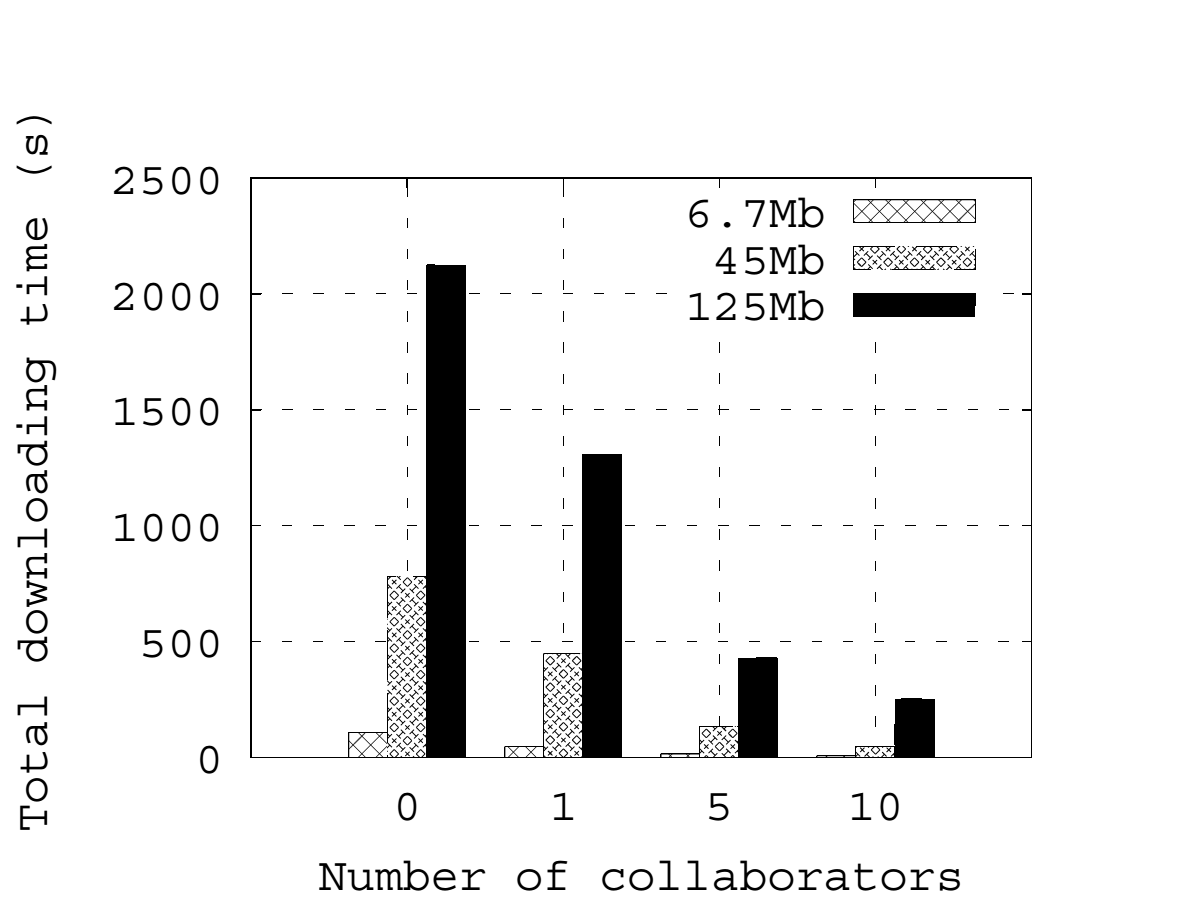
\includegraphics[scale=.275]{figures/Results.png}
\end{figure}
\end{frame}
\subsection{Discussion}
\begin{frame}
\frametitle{Discussion}
\begin{itemize}
\item Content Filtering (Copy righted materials)
\begin{itemize}
\item Onion routing
\end{itemize}
\item Privacy
\begin{itemize}
\item Can I see what the initiator watch
\item What usage information the initiator will have about collaborators.
\end{itemize}
\item Security
\begin{itemize}
\item Built in man in the middle???
\item Handling unknown data for anonymous person !!!!
\end{itemize}
\end{itemize}
\end{frame}

\begin{frame}
\frametitle{Questions?}
\begin{figure}[hbtp]
\centering

\includegraphics[scale=.1]{figures/question-mark-nothing.jpg}
\end{figure}
\end{frame}

\begin{frame}
\frametitle{References}
\begin{enumerate}
\item ColStream: Collaborative Streaming of On-Demand Videos for Mobile Devices
\begin{itemize}
\item Mingyang Zhong, Peizhao Hu, Jadwiga Indulska, Mohan J Kumar
\end{itemize}
\item Mobilnetze, dienstintegrierte Netze und Echtzeitkommunikation. Chapter 1
\begin{itemize}
\item Prof. Dr. rer. nat. Bernd E. Wolfinger
\end{itemize}
\item Cisco visual networking index: Global mobile data traffic forecast update, 20122017, Cisco white paper, Feb 2013.
\end{enumerate}
\end{frame}

%\section{Extended Results}
%\begin{frame}
%\frametitle{Scenarios}
%\end{frame}
%\begin{frame}
%\frametitle{Results}
%\end{frame}
\end{document}
